\section{Affine minima with arbitrary tolerance}
\label{sec:affine}

The proof will use a finite minimum of affine functions on the positive
orthant. Its essential property is that an active slope approximates the
exponent vector of the point where it is active. The allowed error will
depend on the slope and may be discontinuous. We prove the construction
and its uniform consequence from
\cite[Lemma~2.1 and Corollary~2.2]{OpenAI2026} in full.

For $m\geq1$, $u\in\R^m$, and $0<h<1$, put
\[
 X_h(u)=(h^{u_1},\ldots,h^{u_m}).
\]
A \emph{label} $\lambda=(r_\lambda,b_\lambda)$ consists of a slope
$r_\lambda\in\R^m$, independent of $h$, and an offset $b_\lambda(h)$
defined for all sufficiently small positive $h$. For a finite nonempty
family $\Lambda$ of labels, write
\[
 F_h(x)=\min_{\lambda\in\Lambda}
       \bigl(r_\lambda\cdot x+b_\lambda(h)\bigr).
\]
A label is \emph{active at $x$} if its affine value equals $F_h(x)$.
Every minimizing label is active when there is a tie. All offsets in a
finite family are understood to be restricted to a common interval on
which they are defined.

\begin{lemma}[Affine approximation with arbitrary tolerance]
\label{lem:affine}
Let $m\geq1$ be an integer, let $a<b$ be real numbers, and let
$E:[a,b]^m\to(0,\infty)$ be any function. There is a finite nonempty
family $\Lambda$ of labels with
\[
 r_\lambda\in[a,b]^m,
 \qquad b_\lambda(h)=o(h^a)\quad(h\to0+),
\]
such that the following implication holds. If $h_\nu\to0+$,
$p^\nu\in\R^m$ converges to $p\in[a,b]^m$, and a fixed label
$\lambda\in\Lambda$ is active at $X_{h_\nu}(p^\nu)$ for every $\nu$,
then
\[
 \norm{p-r_\lambda}_\infty<E(r_\lambda).
\]
The slopes and the family are independent of $h$. No regularity is
assumed of $E$, and the approximating vectors $p^\nu$ need not lie in
$[a,b]^m$.
\end{lemma}

\begin{proof}
We induct on $m$. Write $\mu(u)=\min_i u_i$ and
$\one=(1,\ldots,1)$. Since the largest coordinate of $X_h(u)$ is
$h^{\mu(u)}$, we first construct a family for each fixed value $t$ of
the smallest exponent. We then extend its guarantee to a neighborhood
of $t$ and combine finitely many such families by shifting their offsets.
The fixed-minimum construction is a singleton when $m=1$; the extension
and combination therefore also prove the base case.

Throughout the proof, asymptotic comparisons along $h_\nu\to0+$ and
$p^\nu\to p$ use fixed gaps between limiting exponents. In particular,
if $p_i>q$, then eventually $p_i^\nu\geq q+\delta$ for some
$\delta>0$, so $h_\nu^{p_i^\nu}=o(h_\nu^q)$; if $p_i<q$, the ratio
$h_\nu^{p_i^\nu}/h_\nu^q$ tends to infinity. We shall use these
comparisons only with strict limiting gaps.

\medskip
\noindent\emph{A family for a fixed minimum.}
Fix $t\in[a,b]$. We construct a finite family $\Lambda_t$ containing
$(t\one,0)$, with $\mu(r)=t$ for every slope, such that the conclusion
of the lemma holds for activity within $\Lambda_t$ whenever
$\mu(p)=t$.

If $m=1$ or $t=b$, the family $\{(t\one,0)\}$ suffices: a point
$p\in[a,b]^m$ with $\mu(p)=t$ then equals $t\one$. Otherwise
$m>1$ and $t<b$. Say a label has \emph{type $k$} if exactly $k$
entries of its slope exceed $t$, the remaining entries being $t$.
Start with the type~$0$ label $(t\one,0)$, and construct types
$k=1,\ldots,m-1$ successively. After type~$k-1$ has been constructed,
choose $\beta_k$ satisfying
\begin{gather*}
 t<\beta_k<b,\qquad
 \beta_k<\beta_{k-1}\quad\text{if }k>1,\\
 \beta_k-t<E(r)
 \quad\text{for every slope $r$ of type $k-1$.}
\end{gather*}
These conditions use only finitely many positive values of $E$, so
such a choice is possible. The new type~$k$ labels will force every
limiting exponent on a coordinate left at $t$ by a type~$k-1$ label
that stays active to be at most $\beta_k$. The last inequality will
then bound the error by that label's tolerance.

For each $k$-element coordinate set $U\subset\{1,\ldots,m\}$ and
$s\in[\beta_k,b]^U$, let $r(s)$ equal $s$ on $U$ and $t$ off $U$.
Apply the induction hypothesis in dimension $k$ to this cube with
tolerance $s\mapsto E(r(s))$, identifying $U$ with its naturally ordered
coordinates. For every resulting label $(s,d)$, add to $\Lambda_t$ the
type~$k$ label
\begin{equation}
 r=r(s),\qquad c(h)=-h^{\beta_k}+d(h),
 \qquad d(h)=o(h^{\beta_k}).
 \label{eq:local-labels}
\end{equation}
Here and below $c$ denotes a local offset. The resulting family is finite,
and all its offsets are $o(h^t)$. The negative offset favors raising
slope entries on coordinates where $X_h(p)$ is small; the decreasing
$\beta_k$ make that preference stronger with each successive type.

To verify the guarantee, let $p^\nu\to p\in[a,b]^m$ with
$\mu(p)=t$, and suppose a type~$k$ label $(r,c)$ stays active within
$\Lambda_t$ along $h_\nu\to0+$. Let $U$ be its raised coordinate set,
and abbreviate $h=h_\nu$. For $k>0$, comparison with $(t\one,0)$
gives
\[
 \sum_{i\in U}(r_i-t)h^{p_i^\nu}
 \leq h^{\beta_k}-d(h)=(1+o(1))h^{\beta_k}.
\]
Every coefficient on the left is at least $\beta_k-t>0$. A limiting
exponent $p_i<\beta_k$ would make the corresponding term divided by
$h^{\beta_k}$ tend to infinity. Therefore
\begin{equation}
 p_i\geq\beta_k\qquad(i\in U).
 \label{eq:raised-coordinates}
\end{equation}
Among labels made from this same $U$, all contributions off $U$ and
the term $-h^{\beta_k}$ are common. Thus $(s,d)$ is active in the
family furnished by induction. Its limiting exponent vector lies in
$[\beta_k,b]^U$, so
\[
 \max_{i\in U}\abs{p_i-r_i}<E(r).
\]
The approximating vectors $p_U^\nu$ may approach a face of that cube
from outside. This is why the induction statement allows them outside
the cube, including when $p_i=\beta_k$ or $p_i=b$.

It remains to bound the coordinates off $U$. This argument also includes
type~$0$, for which $U=\varnothing$. If $k<m-1$, we claim that
\[
 p_i\leq\beta_{k+1}\qquad(i\notin U).
\]
Otherwise choose $j\notin U$ with $p_j>\beta_{k+1}$ and any
type~$k+1$ label raised on $U\cup\{j\}$. Every limiting exponent
on this set exceeds $\beta_{k+1}$, by
\eqref{eq:raised-coordinates} and $\beta_k>\beta_{k+1}$ when
$k>0$. The competitor's affine value minus that of $(t\one,0)$ is
therefore
\[
 -h^{\beta_{k+1}}+o(h^{\beta_{k+1}}).
\]
For the supposed active label, the same difference is zero if $k=0$,
and is bounded below by $-h^{\beta_k}+o(h^{\beta_k})$ if $k>0$.
Since $h^{\beta_k}=o(h^{\beta_{k+1}})$, the competitor is strictly
smaller for all sufficiently small $h$ along the sequence, a
contradiction. Consequently, off $U$,
\[
 \abs{p_i-r_i}\leq\beta_{k+1}-t<E(r).
\]
If $k=m-1$, there is just one coordinate off $U$. Its limiting exponent
is $t$, since $\mu(p)=t$ and all coordinates on $U$ have limiting
exponents greater than $t$. Its error is zero. This proves the required
strict bound for every active label at the fixed minimum.

\medskip
\noindent\emph{Extension to nearby minima.}
For a fixed label $\lambda=(r,c)\in\Lambda_t$, let
$A_\lambda\subset[a,b]^m$ consist of the limits of all sequences
$p^\nu\in\R^m$ for which $h_\nu\to0+$ and $\lambda$ is active
within $\Lambda_t$ at $X_{h_\nu}(p^\nu)$. This set is closed.
Indeed, if $z_n\in A_\lambda$ and $z_n\to z$, choose from a
sequence realizing $z_n$ a parameter $0<h_n<1/n$ and a vector $u_n$
with $\norm{u_n-z_n}_\infty<1/n$ such that $\lambda$ is active at
$X_{h_n}(u_n)$.
Then $u_n\to z$, so this selected sequence realizes $z\in A_\lambda$.
This argument uses actual active points and requires no continuity of
the offsets in $h$.

The set of limits violating the desired estimate,
\[
 B_t=\bigcup_{\lambda=(r,c)\in\Lambda_t}
 \{p\in A_\lambda:\norm{p-r}_\infty\geq E(r)\},
\]
is compact: the union is finite and each $E(r)$ here is a fixed number.
The preceding argument shows that $B_t$ contains no point with
$\mu(p)=t$. Continuity of $\mu$ and compactness therefore give
$\rho_t>0$ such that $B_t$ contains no point with
\[
 \mu(p)\in I_t:=(t-\rho_t,t+\rho_t).
\]
If $B_t$ is empty any positive radius initially suffices; otherwise take
$\rho_t<\min_{p\in B_t}\abs{\mu(p)-t}$. Thus $\Lambda_t$
has the asserted limiting activity property whenever $\mu(p)\in I_t$.

Shrink $\rho_t$ further, if necessary, so that every local offset obeys
\begin{equation}
 c(h)=o(h^{t+\rho_t}).
 \label{eq:local-decay}
\end{equation}
For a nonsingleton family, choose $t+\rho_t<\min_k\beta_k$ and use
\eqref{eq:local-labels}; for a singleton the offset is zero.
We have obtained a family valid near each possible minimum exponent.
The remaining task is to ensure that a globally active label comes from
a family valid at its own limiting point.

\medskip
\noindent\emph{Combining the families.}
Take a finite subcover of $[a,b]$ from the intervals $I_t$. Discard
intervals contained in others, keeping just one if two coincide, and
order the remaining centers as $t_1<\cdots<t_N$. Write
$I_{t_j}=(L_j,R_j)$. Noncontainment forces both endpoints to have the
same strict order; since $t_j=(L_j+R_j)/2$, it is the order of the
centers. Hence
\[
 L_1<\cdots<L_N,\qquad R_1<\cdots<R_N.
\]
Consecutive intervals overlap. If $R_j\leq L_{j+1}$, a point of
$[R_j,L_{j+1}]\subset(t_j,t_{j+1})\subset[a,b]$ would be uncovered.
The first interval contains $a$ and the last contains $b$.

For $1\leq j<N$, choose a cut
\[
 q_j\in
 \bigl(\max\{t_j,L_{j+1}\},\min\{t_{j+1},R_j\}\bigr).
\]
The interval displayed is nonempty because consecutive intervals overlap
and each contains its own center. With $q_0=a$ and $q_N=b$, we have
\begin{equation}
 t_j<q_j<t_{j+1}\quad(1\leq j<N),
 \qquad [q_{j-1},q_j]\subset I_{t_j}\quad(1\leq j\leq N).
 \label{eq:affine-cuts}
\end{equation}
For $N=1$, the sole interval contains $[a,b]$ and no interior cuts are
needed. The closed intervals in \eqref{eq:affine-cuts} are the ranges
of minimum exponents assigned to the respective families; see
Figure~\ref{fig:intervals}.

Combine the selected families, replacing every local offset $c(h)$ in
$\Lambda_{t_j}$ by
\begin{equation}
 \widetilde c(h)=c(h)-\sum_{\ell=1}^{j-1}h^{q_\ell}.
 \label{eq:affine-shifts}
\end{equation}
These offsets are $o(h^a)$: \eqref{eq:local-decay} has
$t_j+\rho_{t_j}>a$, and each shift exponent satisfies
$q_\ell>t_\ell\geq a$. A common shift preserves activity within each
family. Between consecutive families, the new term $-h^{q_j}$ will
force any limiting minimum exponent to the correct side of the cut.

\begin{figure}[tb]
\centering
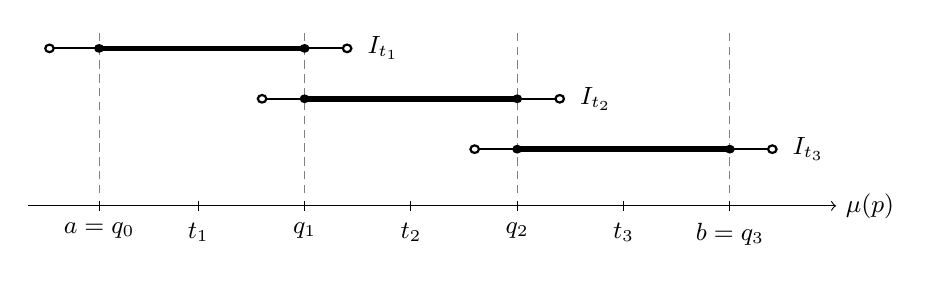
\begin{tikzpicture}[x=0.9cm,y=0.8cm,font=\small]
  \draw[->,thin] (-0.4,0) -- (11.0,0) node[right] {$\mu(p)$};
  \foreach \x/\label in {0.6/{a=q_0},2/{t_1},3.5/{q_1},5/{t_2},6.5/{q_2},8/{t_3},9.5/{b=q_3}} {
    \draw (\x,0.08) -- (\x,-0.08);
    \node[below] at (\x,-0.12) {$\label$};
  }
  \foreach \x in {0.6,3.5,6.5,9.5} {
    \draw[gray,densely dashed,thin] (\x,0.2) -- (\x,2.75);
  }
  \draw[thick] (-0.1,2.5) -- (4.1,2.5);
  \draw[fill=white,thick] (-0.1,2.5) circle (0.06);
  \draw[fill=white,thick] (4.1,2.5) circle (0.06);
  \draw[line width=2pt] (0.6,2.5) -- (3.5,2.5);
  \fill (0.6,2.5) circle (0.07);
  \fill (3.5,2.5) circle (0.07);
  \node[right] at (4.25,2.5) {$I_{t_1}$};
  \draw[thick] (2.9,1.7) -- (7.1,1.7);
  \draw[fill=white,thick] (2.9,1.7) circle (0.06);
  \draw[fill=white,thick] (7.1,1.7) circle (0.06);
  \draw[line width=2pt] (3.5,1.7) -- (6.5,1.7);
  \fill (3.5,1.7) circle (0.07);
  \fill (6.5,1.7) circle (0.07);
  \node[right] at (7.25,1.7) {$I_{t_2}$};
  \draw[thick] (5.9,0.9) -- (10.1,0.9);
  \draw[fill=white,thick] (5.9,0.9) circle (0.06);
  \draw[fill=white,thick] (10.1,0.9) circle (0.06);
  \draw[line width=2pt] (6.5,0.9) -- (9.5,0.9);
  \fill (6.5,0.9) circle (0.07);
  \fill (9.5,0.9) circle (0.07);
  \node[right] at (10.25,0.9) {$I_{t_3}$};
\end{tikzpicture}
\caption{Combining three local families, schematically. Each thick closed
interval $[q_{j-1},q_j]$ lies inside the open neighborhood $I_{t_j}$
where its family is valid. The shifts in \eqref{eq:affine-shifts} force
the limiting minimum exponent of an active label into this closed
interval. At a cut, either neighboring family remains valid.}
\label{fig:intervals}
\end{figure}


Suppose a fixed label from $\Lambda_{t_j}$ is active in the combined
family along $h_\nu\to0+$ and $p^\nu\to p\in[a,b]^m$. Write
$c(h)$ for its original local offset and $h=h_\nu$. We claim
\[
 q_{j-1}\leq\mu(p)\leq q_j.
\]
If $j<N$ and $\mu(p)>q_j$, each coordinate $h^{p_i^\nu}$ is
$o(h^{q_j})$. Also $c(h)=o(h^{q_j})$, by
\eqref{eq:local-decay} and $q_j<R_j=t_j+\rho_{t_j}$. Subtracting
the value of the shifted label $(t_{j+1}\one,0)$ from the active
label's value gives
\[
 (r-t_{j+1}\one)\cdot X_h(p^\nu)+c(h)+h^{q_j}
   =h^{q_j}+o(h^{q_j})>0,
\]
a contradiction.

If $j>1$ and $\mu(p)<q_{j-1}$, compare instead with the shifted
label $(t_{j-1}\one,0)$. The difference is
\[
 (r-t_{j-1}\one)\cdot X_h(p^\nu)+c(h)-h^{q_{j-1}}.
\]
Every coefficient in the scalar product is at least
$t_j-t_{j-1}>0$. Some coordinate has $p_i<q_{j-1}$, so its
exponential divided by $h^{q_{j-1}}$ tends to infinity. Meanwhile,
$c(h)=o(h^{q_{j-1}})$ because $q_{j-1}<t_j<t_j+\rho_{t_j}$.
Thus the displayed difference divided by $h^{q_{j-1}}$ tends to
$+\infty$, again contradicting activity. The outer bounds for $j=1$
or $j=N$ follow from $\mu(p)\in[a,b]$.

By \eqref{eq:affine-cuts}, the claimed bounds place $\mu(p)$ inside
$I_{t_j}$, including when it equals a cut. The label is active within
its original local family, so the guarantee on $I_{t_j}$ gives
$\norm{p-r}_\infty<E(r)$. This completes the induction.
\end{proof}

The sequential formulation yields the uniform statement needed below.
Its order of choices is important: the family, and hence its finite set
of slopes, is fixed before the upper bound on $h$ is chosen.

\begin{corollary}[Uniform activity bound]
\label{cor:activity}
Let $m\geq1$, $a<b$, and $E:[a,b]^m\to(0,\infty)$ be as in
Lemma~\ref{lem:affine}. Fix a family $\Lambda$ supplied by that
lemma. There is $h_0\in(0,1)$ such that, for every $0<h<h_0$ and
every $p\in[a,b]^m$, each label $\lambda\in\Lambda$ active at
$X_h(p)$ satisfies
\[
 \norm{p-r_\lambda}_\infty<E(r_\lambda).
\]
\end{corollary}

\begin{proof}
Otherwise there are $h_\nu\to0+$, points $p^\nu\in[a,b]^m$, and
active labels $\lambda_\nu$ such that
$\norm{p^\nu-r_{\lambda_\nu}}_\infty\geq E(r_{\lambda_\nu})$.
By finiteness and compactness, pass to a subsequence on which
$\lambda_\nu=\lambda$ is fixed and $p^\nu\to p\in[a,b]^m$.
The inequality passes to the limit and contradicts
Lemma~\ref{lem:affine}. No continuity of $E$ is needed because its
argument $r_\lambda$ is fixed on this subsequence.
\end{proof}
